\documentclass[cs4size,a4paper]{ctexart}   
%==================== 数学符号公式 ============
\usepackage{amsmath}                 % AMS LaTeX宏包
\usepackage[style=1]{mdframed}
\usepackage{amsthm}
\usepackage{amsfonts}
\usepackage{mathrsfs}                % 英文花体字 体
\usepackage{bm}                      % 数学公式中的黑斜体
\usepackage{bbding,manfnt}           % 一些图标,如 \dbend
\usepackage{lettrine}                % 首字下沉,命令\lettrine
\def\attention{\lettrine[lines=2,lraise=0,nindent=0em]{\large\textdbend\hspace{1mm}}{}}
\usepackage{longtable}
\usepackage[toc,page]{appendix}
\usepackage{geometry}                % 页边距调整
\geometry{top=3.0cm,bottom=2.7cm,left=2.5cm,right=2.5cm}
%====================公式按章编号==========================
\numberwithin{equation}{section}
\numberwithin{table}{section}
\numberwithin{figure}{section}
%================= 基本格式预置 ===========================
\usepackage{fancyhdr}
\pagestyle{fancy}
\fancyhf{}  
\fancyhead[C]{\zihao{5}  \kaishu 数字电路与逻辑设计课程大作业}
\fancyfoot[C]{~\zihao{5} \thepage~}
\renewcommand{\headrulewidth}{0.65pt} 
\CTEXsetup[format={\centering\bfseries\zihao{-2}},name={第, 章}]{section}
\CTEXsetup[nameformat={\bfseries\zihao{3}}]{subsection}
\CTEXsetup[nameformat={\bfseries\zihao{4}}]{subsubsection}
%================== 图形支持宏包 =========================
\usepackage{subfigure}
\usepackage{graphicx}                % 嵌入png图像
\usepackage{color,xcolor}            % 支持彩色文本、底色、文本框等
\usepackage{hyperref}                % 交叉引用
\usepackage{caption}
\captionsetup{figurewithin=section}
%===================== 超链接 ========================
\usepackage{hyperref}
%==================== 源码和流程图 =====================
\usepackage{listings}                % 粘贴源代码
\usepackage{xcolor}
\usepackage{color}
\definecolor{dkgreen}{rgb}{0,0.6,0}
\definecolor{gray}{rgb}{0.5,0.5,0.5}
\definecolor{mauve}{rgb}{0.58,0,0.82}
\usepackage{xcolor}
\lstset{
	%行号
	numbers=left,
	%背景框
	framexleftmargin=8mm,
	frame=none,
	%背景色
	%backgroundcolor=\color[rgb]{1,1,0.76},
	backgroundcolor=\color[RGB]{245,245,244},
	%样式
	keywordstyle=\bf\color{blue},
	identifierstyle=\bf,
	numberstyle=\color[RGB]{0,192,192},
	commentstyle=\it\color[RGB]{0,96,96},
	stringstyle=\rmfamily\slshape\color[RGB]{128,0,0},
	% 显示空格
	showstringspaces = false,
	% 自动换行
	breaklines = true
}

% 表格
\usepackage{booktabs}

%--------------------
\hypersetup{hidelinks}
\usepackage{booktabs}  
\usepackage{shorttoc}
\usepackage{tabu,tikz}
\usepackage{float}

\usepackage{multirow}
\usepackage{enumerate}


\tabcolsep=1ex
\tabulinesep=\tabcolsep
\newlength\tikzboxwidth
\newlength\tikzboxheight
\newcommand\tikzbox[1]{%
	\settowidth\tikzboxwidth{#1}%
	\settoheight\tikzboxheight{#1}%
	\begin{tikzpicture}
	\path[use as bounding box]
	(-0.5\tikzboxwidth,-0.5\tikzboxheight)rectangle
	(0.5\tikzboxwidth,0.5\tikzboxheight);
	\node[inner sep=\tabcolsep+0.5\arrayrulewidth,line width=0.5mm,draw=black]
	at(0,0){#1};
	\end{tikzpicture}%
}

\makeatletter
\def\hlinew#1{%
	\noalign{\ifnum0=`}\fi\hrule \@height #1 \futurelet
	\reserved@a\@xhline}

\newcommand{\tabincell}[2]{\begin{tabular}{@{}#1@{}}#2\end{tabular}}%

\usepackage{subfigure}

\usepackage{CJK}
\usepackage{ifthen}


\usepackage{graphicx} 
\newcommand{\HRule}{\rule{\linewidth}{0.5mm}}

\newtheorem{Theorem}{定理}
\newtheorem{Lemma}{引理} 
%%使得公式随章节自动编号
\makeatletter
\@addtoreset{equation}{section}
\makeatother
\renewcommand{\theequation}{\arabic{section}.\arabic{equation}}

%-------------------------

\usepackage{pythonhighlight}
\usepackage{tikz}                    
\usepackage{tikz-3dplot}
\usetikzlibrary{shapes,arrows,positioning}
%===================   正文开始    ===================
\begin{document}
	% \bibliographystyle{gbt7714-2005}     %论文引用格式
	% \bibliographystyle{plain} % 字母顺序
	\bibliographystyle{unsrt}
	%===================  定理类环境定义 ===================
	\newtheorem{example}{例}              % 整体编号
	\newtheorem{algorithm}{算法}
	\newtheorem{theorem}{定理}            % 按 section 编号
	\newtheorem{definition}{定义}
	\newtheorem{axiom}{公理}
	\newtheorem{property}{性质}
	\newtheorem{proposition}{命题}
	\newtheorem{lemma}{引理}
	\newtheorem{corollary}{推论}
	\newtheorem{remark}{注解}
	\newtheorem{condition}{条件}
	\newtheorem{conclusion}{结论}
	\newtheorem{assumption}{假设}
	%==================重定义 ===================
	\renewcommand{\contentsname}{目录}     
	\renewcommand{\abstractname}{摘要} 
	\renewcommand{\refname}{参考文献}     
	\renewcommand{\indexname}{索引}
	\renewcommand{\figurename}{图}
	\renewcommand{\tablename}{表}
	\renewcommand{\appendixname}{附录}
	\renewcommand{\proofname}{证明}
	\renewcommand{\algorithm}{算法} 
	%============== 封皮和前言 =================
	\begin{titlepage}

\begin{center}


% Upper part of the page

\includegraphics[width=0.65\textwidth]{figure/logo_xdred}\\[1cm]    

\textsc{\LARGE \bfseries 人工智能学院}\\[1.5cm]

\textsc{\Large 概率论与数理统计课程大作业报告}\\[0.5cm]


% Title
\HRule \\[0.4cm]
{ \huge \bfseries 三门问题的分析与解}\\[0.4cm]

\HRule \\[1.5cm]

% Author and supervisor
\begin{minipage}{0.4\textwidth}
\begin{center} \large
%\emph{Author:}\\
\textsc {\kaishu 姓名:杨文韬\\学号:18020100245\\班级: 1920012}
\end{center}
\end{minipage}
%\begin{minipage}{0.4\textwidth}
%\begin{flushright} \large
%\emph{Supervisor:} \\
%Dr.~Mark \textsc{Brown}
%\end{flushright}
%\end{minipage}

\vfill

% Bottom of the page
% {\large \today}
{\large 2020年12月24日}

\end{center}

\end{titlepage}

	\pagestyle{plain}
	\pagenumbering{Roman}
	% \section*{\zihao{2} \centering 摘要}

\vskip0.5cm
本文介绍了三门问题的背景,从一位学者的论文中找出错误,即结果与主持人打开有山羊门的概率无关,而是与主持人是否只会选择山羊门打开有关。通过枚举法、贝叶斯公式和蒙特卡罗方法模拟得到了正确的结论,蒙特卡罗方法是一种统计模拟方法,采样越多,越近似最优解,笔者用 MATLAB 自己编写算法实现了蒙特卡罗方法,并对其进行了可视化展示,并得出一致结论:在主持人每次选择羊的门打开的情况下,选手坚持策略赢得车的概率为 $\frac{1}{3}$,而换门策略赢得汽车的概率为 $\frac{2}{3}$,故选手需要改变策略,在文章的最后,给出了一些思考与总结,指出很多悖论的产生都是因为条件限制而引起的。

\textbf{关键词:}  枚举法,条件概率,贝叶斯公式,蒙特卡罗方法,悖论 
% \addcontentsline{toc}{section}{摘要}

% \clearpage
% \section*{\zihao{2} \centering \textbf{Abstract} }
%   %用了Times New Roman字体来美化观感

% Support vector machine (SVM) is a new pattern recognition method developed on the basis of statistical learning theory. It shows many unique advantages in solving small sample, nonlinear and high-dimensional pattern recognition problems. Handwritten digit recognition is one of the research hotspots with high practical value in image processing and pattern recognition. The MNIST database (Mixed National Institute of Standards and Technology database) is a large database of handwritten digits, usually used to train various image processing systems. The database is also widely used for training and testing in the field of machine learning. In this paper, the SVM kernel method is used, and the kernel functions such as RBF kernel, linear kernel, Sigmoid kernel and customized second-order norm kernel are used to realize the handwritten digit recognition function. The results show that the accuracy of model recognition obtained by RBF kernel is more than 98\%, which is more satisfactory than other kernel methods. \\

% \textbf{Key Words:} SVM, Handwritten Digit Recognition, Kernel Function
\addcontentsline{toc}{section}{摘要}





	\pagestyle{empty}
	\tableofcontents 
	\thispagestyle{empty}
	%============== 论文正文   =================
	\pagestyle{fancy}
	\pagenumbering{arabic}
\section{概述}

\subsection{简述}

数字电子钟是一种用数字显示秒、分、时、日的计时装置,与传统的机械钟相比,它具有走时准确,显示直观、无机械传动装置等优点,因而得到了广泛的应用。小到人们日常生活中的电子手表,大到车站、码头、机场等公共场所的大型数显电子钟。

数字电子钟由以下几部分组成:石英晶体振荡器和分频器组成的秒脉冲发生器;校时电路;六十进制秒、分计数器,二十四进制(或十二进制)计时计数器;秒、分、时的译码显示部分等。


\subsection{设计任务和要求}

用中、小规模集成电路设计一台能显示日、时、分、秒的数字电子钟,要求如下:

\begin{enumerate}[1.]
\item 由晶振电路产生1Hz标准秒信号。
\item 秒、分为00~59六十进制计数器。
\item 时为00~23二十四进制计数器。
\item 周显示从1~日为七进制计数器。
\item 可手动校时:能分别进行秒、分、时、日的校时。只要将开关置于手动位置,可分别对秒、分、时、日进行手动脉冲输入调整或连续脉冲输入的校正。
\item 整点报时。整点报时电路要求在每个整点前呜叫五次低音(500Hz),整点时再呜叫一次高音(1000Hz)。
\end{enumerate}

\subsection{设计工具}

\begin{itemize}
	\item Multisim 14.0(电路仿真)
	\item LaTeX(文档编写)
	\item OBS+格式工厂(功能演示视频录制)
	\item Visio 2016(流程图绘制)
\end{itemize}

\subsection{元件清单}

74 系列的元件有以下几种,在我的设计中用的的元件清单如表 \ref{tool} 所示。

\begin{enumerate}[1)]
	\item 74××(标准型)
	\item 74S××(肖特基)
	\item 74LS××(低功耗肖特基)
	\item 74ALS××(先进低功耗肖特基)
	\item 74AS××(先进肖特基)
	\item 74F××(高速)
\end{enumerate}


\begin{table}[hbtp]
	\setlength{\abovecaptionskip}{0cm} 
	\setlength{\belowcaptionskip}{-0.2cm}
	\begin{center}
	\caption{元件清单表}
	\begin{tabular}{|c|p{4cm}<{\centering}|p{2cm}<{\centering}|c|c|}
		\hline
		\textbf{Quantity} & \textbf{Description}  & \textbf{RefDes}               & \textbf{Package}                   & \textbf{Obsolete} \\ \hline
		1                 & TIMER, LM555CM        & U1                            & IPC-7351\textbackslash{}M08A       & No                \\ \hline
		7                 & 74STD, 74160N         & U2, U3, U7, U8, U12, U13, U17 & IPC-2221A/2222\textbackslash{}NO16 & No                \\ \hline
		3                 & 74STD, 7410N          & U6, U11, U16                  & IPC-2221A/2222\textbackslash{}NO14 & No                \\ \hline
		1                 & 74STD, 7427N          & U20                           & IPC-2221A/2222\textbackslash{}NO14 & No                \\ \hline
		4                 & 74STD, 7400N          & U19, U21, U22, U23            & IPC-2221A/2222\textbackslash{}NO14 & No                \\ \hline
		3                 & SPDT,                 & S1, S2, S3                    & Generic\textbackslash{}SPDT        & -                 \\ \hline
		3                 & 74STD, 7451N          & U24, U25, U28                 & IPC-2221A/2222\textbackslash{}NO14 & No                \\ \hline
		4                 & 74STD, 7404N          & U26, U27, U29, U31            & IPC-2221A/2222\textbackslash{}NO14 & No                \\ \hline
		1                 & BUZZER, BUZZER 500Hz  & LS1                           & Generic\textbackslash{}BUZZER      & -                 \\ \hline
		1                 & 74STD, 7408N          & U34                           & IPC-2221A/2222\textbackslash{}NO14 & No                \\ \hline
		1                 & BUZZER, BUZZER 1000Hz & LS2                           & Generic\textbackslash{}BUZZER      & -                 \\ \hline
	\end{tabular} \label{tool}
	\end{center}
\end{table}

\subsection{设计方案流程图}

数字电子钟设计的流程图如图 \ref{fig:FlowChart} 所示。


\begin{figure}[hbtp]
	\centering
	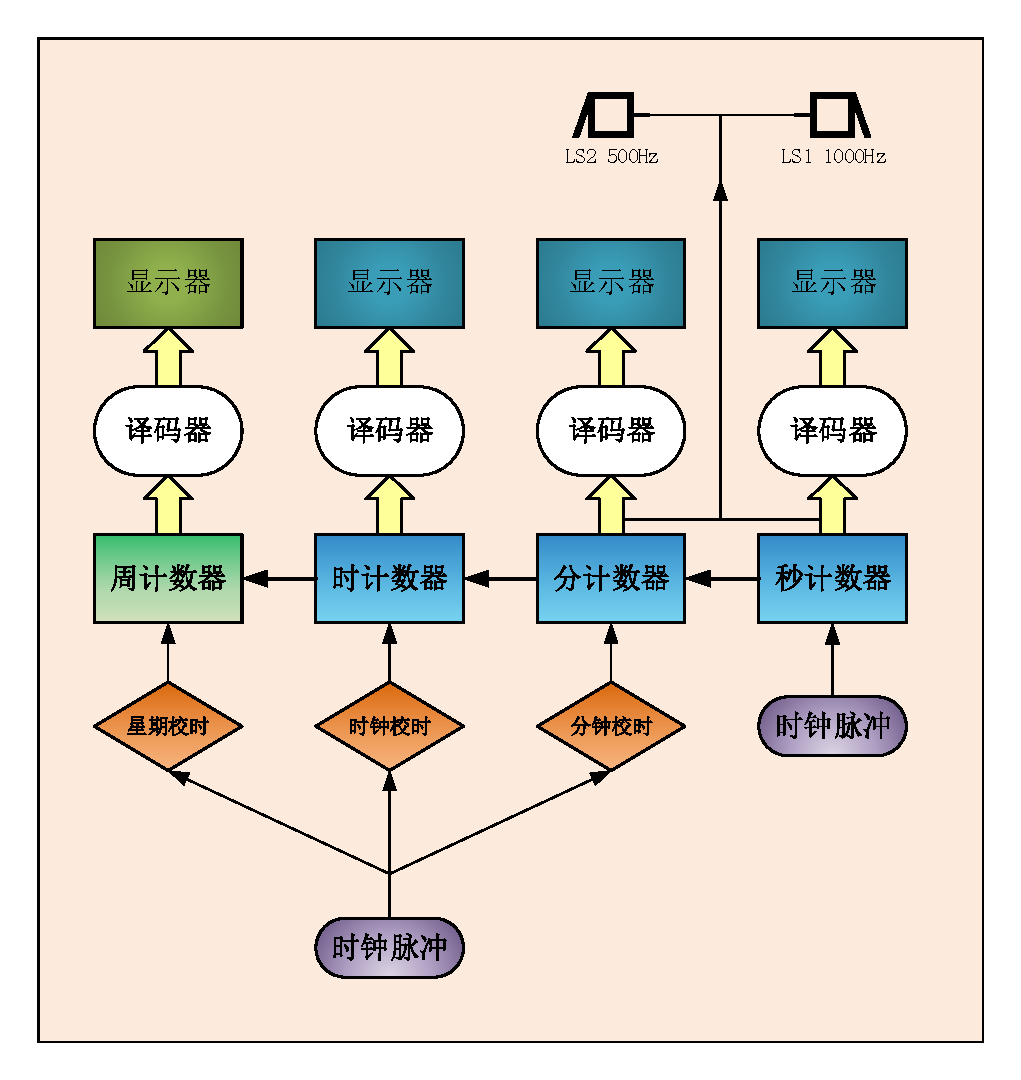
\includegraphics[width=16cm]{figure/FlowChart}
	\caption{设计流程图}\label{fig:FlowChart}
\end{figure}
	\section{理论求解}

\subsection{枚举法}

这里我们假设第一次选择的为第一道门(具有轮换对称性不影响结果),其所有可能结果和最终赢得汽车(用数字 1 表示)的情况如下表所示:

\begin{table}[h]
	\centering
	\begin{tabular}{ccc|cc}
		door 1 & door 2 & door 3 & stick & change \\ \hline
		goat   & goat   & car    & 0     & 1      \\ \hline
		goat   & car    & goat   & 0     & 1      \\ \hline
		car    & goat   & goat   & 1     & 0 
	\end{tabular}
\end{table}

从表中可以看出,改变选择赢得汽车的概率是 $\frac{2}{3}$,而坚持初次选择赢得汽车的概率为 $\frac{1}{3}$。图 \ref{fig:Monty_Tree_Door1} 的树显示了如果玩家最初选择1号门时各种可能结局的可能性。

\begin{figure}[H]
	\centering
	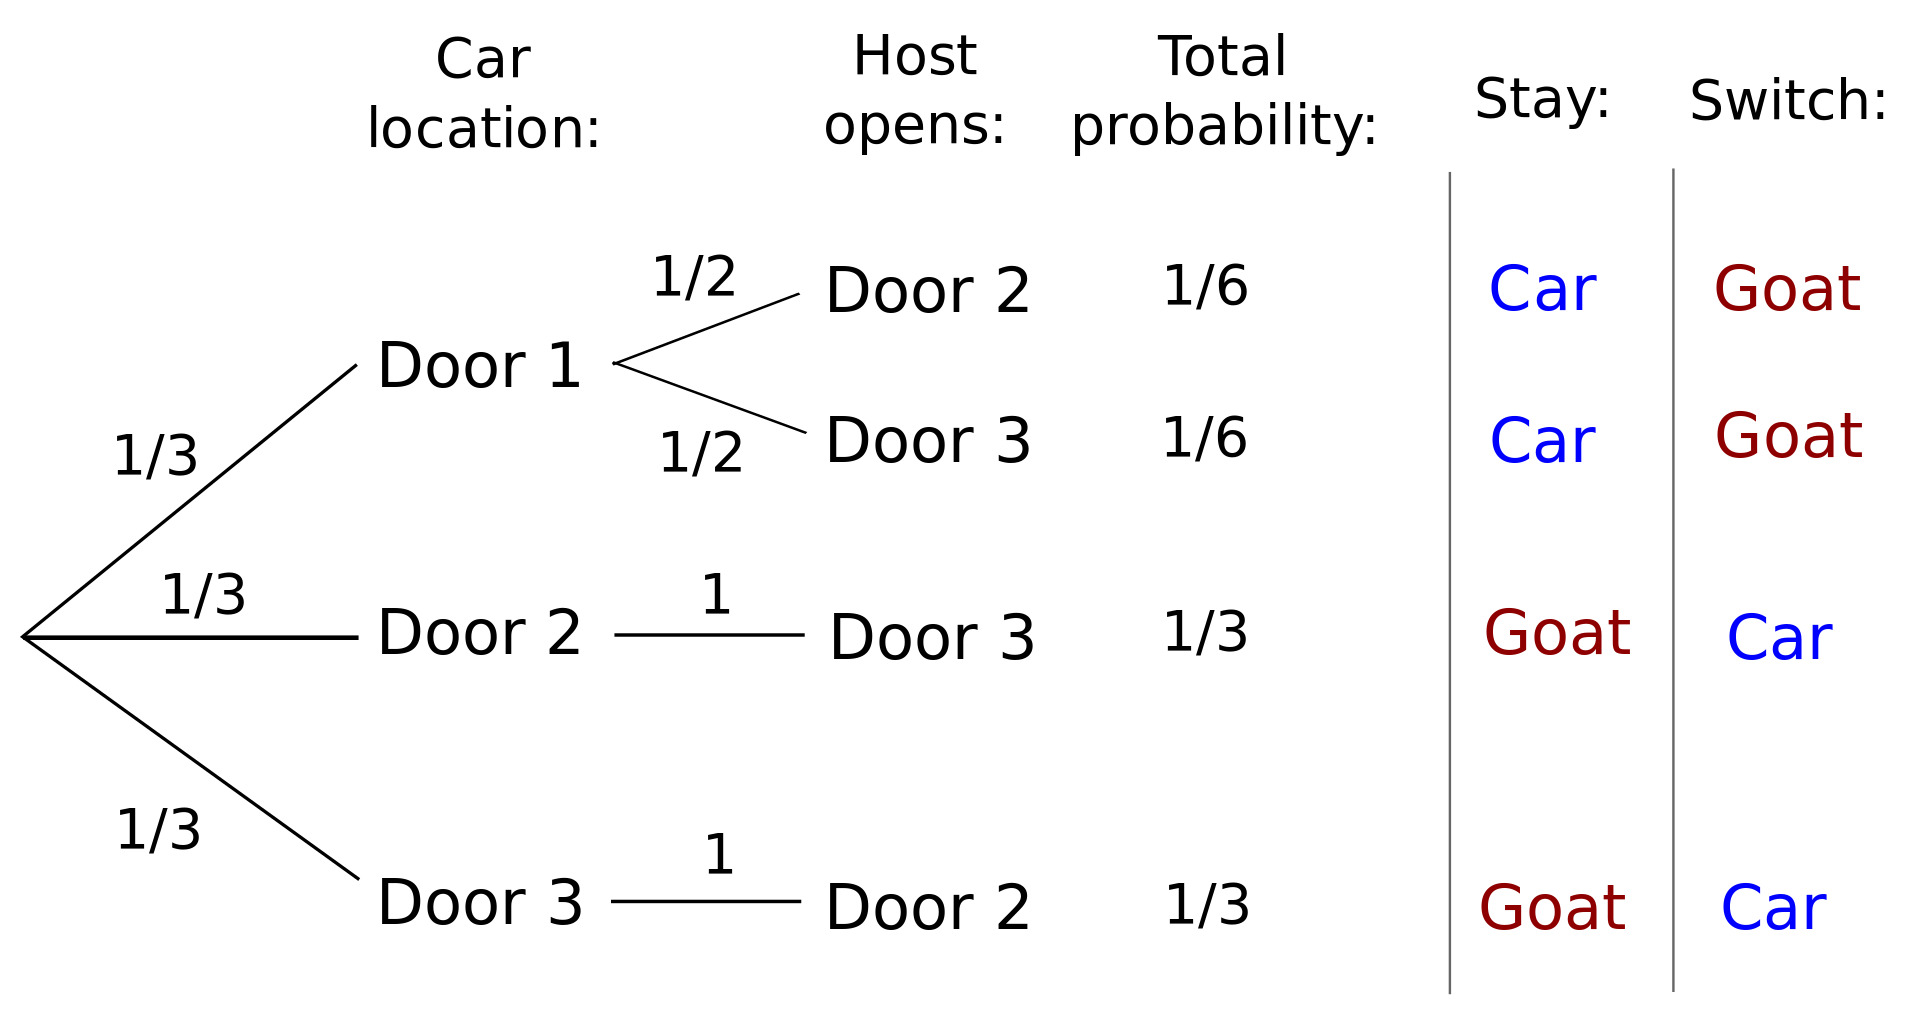
\includegraphics[width=12cm]{figure/tree_door1.jpg}
	\caption{Monty Tree Door1} \label{fig:Monty_Tree_Door1}
\end{figure}

\subsection{概率公式求解}

在上一章中我们给出了两个证明,但其实都包含着同一个错误,即只要主持人选择打开的是含有山羊的门,那么最后得到的结果与主持人打开山羊门的概率无关,即坚持策略获得汽车的概率并非 $P(A_1|B_1C_3)$ 而是 $P(A_1|B_1)$ 或其轮换,改变策略获得汽车的概率并非 $P(A_2|B_1C_3)$ 而是 $P(A_1|B_2)+P(A_1|B_3)$ 或其轮换。

问题的关键在于:主持人知道所有门后面的情况,从而导致了结果违背我们的直觉。

下面给出贝叶斯公式的证明:假设选手选择门 $A$,主持人随后打开 $B$,用 $P(A)$ 表示门 $A$ 后为车,$P(\overline{A})$ 表示 A 后为羊,则选手选择坚持策略获得汽车的概率为 $P(A|\overline{B})$,而选手选择改变策略获得汽车的概率为 $P(\overline{A}|\overline{B})$,下面只计算坚持策略获得汽车概率 $P(A|\overline{B})$,改变策略获得汽车概率为其对立事件,贝叶斯公式如下:

\begin{align*}
P(A|\overline{B})=\frac{P(\overline{B}|A)P(A)}{P(\overline{B}|A)P(A)+P(\overline{B}|\overline{A})P(\overline{A})}
\end{align*}

主持人不会打开有车的门,即 $P(\overline{B}|\overline{A})=1$,另外我们有 $P(A)=\frac{1}{3}$、$P(\overline{A})=\frac{2}{3}$ 和 $P(\overline{B}|A)=1$,代入公式得

\begin{align*}
P(A|\overline{B})=\frac{1\times\frac{1}{3}}{1\times\frac{1}{3}+1\times\frac{2}{3}}=\frac{1}{3}
\end{align*}

故选择坚持策略赢得汽车的概率只有 $\frac{1}{3}$,为了增大概率,应该换门。

假如主持人随意选择一扇门打开,则 $P(\overline{B}|\overline{A})=\frac{1}{2}$,另外我们有 $P(A)=\frac{1}{3}$、$P(\overline{A})=\frac{2}{3}$ 和 $P(\overline{B}|A)=1$,代入公式得

\begin{align*}
P(A|\overline{B})=\frac{1\times\frac{1}{3}}{1\times\frac{1}{3}+\frac{1}{2}\times\frac{2}{3}}=\frac{1}{2}
\end{align*}

可见,如果主持人随机打开一扇门,则换不换门都是一样的概率,因为并没有提供有效信息。

一个更通俗易懂的解释是:当你从三扇门中选择门 A 之后,这扇门后面是车的概率是 $\frac{1}{3}$,门 B 和门 C 有车的概率也是 1/3。但是接下来主持人会给你一个线索。如果奖品在门 B 后面,主持人会打开门 C;如果奖品在门 C 后面,主持人会打开门 B。因此,如果你选择改变策略的话,只要奖品在门 B 或门 C 后你都会赢;但是如果你选择坚持策略,只有奖品在门 A 后你才会赢。


	\section{模拟求解}

\subsection{算法描述}

蒙特卡罗方法(Monte Carlo method),也称统计模拟方法,与它对于的是确定性算法。其基本思想,通过某种“实验”的方法,以这种事件出现的频率估计这一随机事件的概率,或者得到这个随机变量的某些数字特征。

\begin{itemize}
\item \textbf{蒙特卡罗方法}:采样越多,越近似最优解;
\item \textbf{拉斯维加斯方法}:采样越多,越有机会找到最优解。
\end{itemize}

\subsection{代码及结果}

我们用蒙特卡罗算法立即可以写出下面简单的程序:

大概思路是:给出策略和实验次数,进行模拟,每次试验,变量 \verb|car| 和 \verb|first_choice| 分别取随机数初始化车的门和第一次选择的门。如果策略为坚持 \verb|stick|,第一次选择的门为车的门,则赢得汽车次数 \verb|winnings| 进行加一,否则不变;如果策略为改变 \verb|change|,第一次选择的门不为车的门,则赢得汽车次数加一,否则不变。

\lstinputlisting[language=Matlab]{code/Monte_Carlo.m}

得到如下输出

\begin{figure}[H]
	\centering
	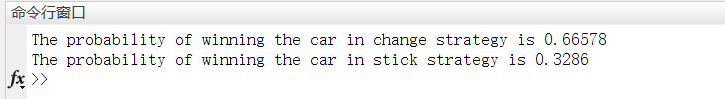
\includegraphics[width=12cm]{figure/out1.png}
\end{figure}

上面这个程序过于简陋了,于是我们利用矩阵重写一个并添加可视化绘图代码如下:

\lstinputlisting[language=Matlab]{code/m_hall.m}

得到如下输出

\begin{figure}[htbp]
	\centering
	\begin{minipage}[t]{0.48\textwidth}
		\centering
		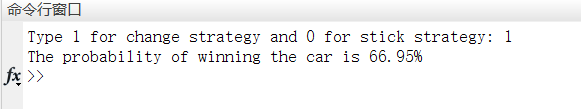
\includegraphics[width=8cm]{figure/out2(1).png}
	\end{minipage}
	\begin{minipage}[t]{0.48\textwidth}
		\centering
		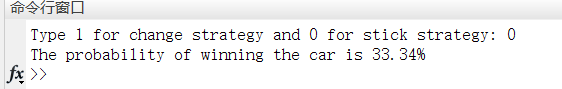
\includegraphics[width=8cm]{figure/out2(2).png}
	\end{minipage}
\end{figure}

绘图结果为:

\begin{figure}[htbp]
	\centering
	\begin{minipage}[t]{0.48\textwidth}
		\centering
		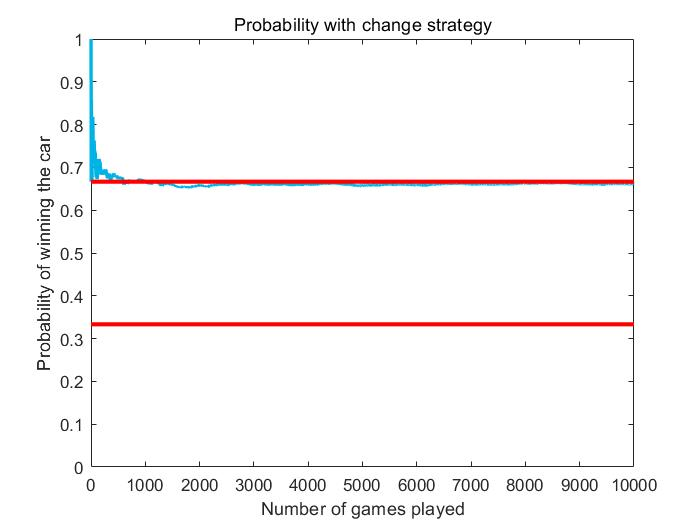
\includegraphics[width=8cm]{figure/change.jpg}
		\caption{Probability with change strategy}
	\end{minipage}
	\begin{minipage}[t]{0.48\textwidth}
		\centering
		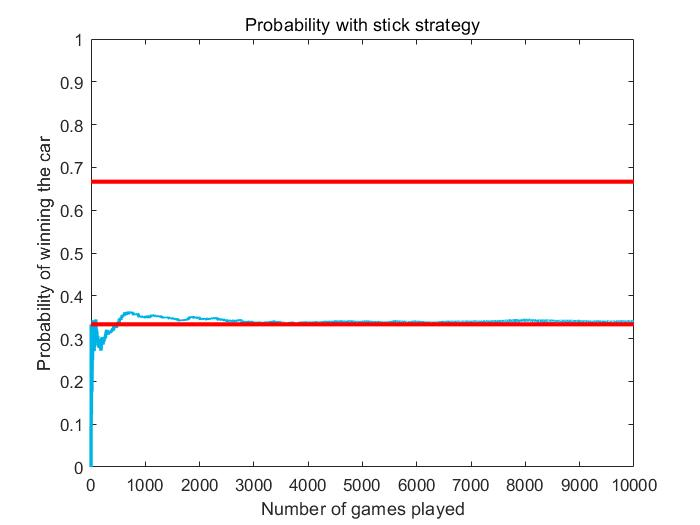
\includegraphics[width=8cm]{figure/stick.jpg}
		\caption{Probability with stick strategy}
	\end{minipage}
\end{figure}
	% \section{思考与总结}

\subsection{一些思考}

三门问题实际上是一个非常简单的问题,主持人认为概率是 $\frac{1}{2}$ 可能是下面的原因:主持人直观地认为排除一羊后通过观察得换不换赢得汽车的概率为 $\frac{1}{2}$,即两门后一羊一车,随机赢得汽车概率为 $\frac{1}{2}$。有心理学家指出,不转换的行为可以用心理学现象解释为:

\begin{itemize}
	\item \textbf{禀赋效应(Endowment effect)}: 当个人一旦拥有某项物品,那么他对该物品价值的评价要比未拥有之前大大提高。也就是说人们往往会高估已选的中奖概率。 
	\item \textbf{现状偏见(Status quo bias)}: 即使改变现状更有利,也不愿改变的心理。也就是说人们更愿意坚持已经做出的选择。
	\item 在所有其他条件相同的情况下,人们更喜欢通过无为(Stay)而不是行动(Switch)来犯错。
\end{itemize}

还可以扩展到更多门的情况,假设有 $N$ 扇门,其中一扇门后有车,其余全为羊。则在主人打开 $M$ 扇有羊的门后选手选择更换策略赢得汽车的概率为 $\frac{N-1}{N(N-M-1)}$ ,这是因为车在其余 $N-1$ 扇门中的一个的概率为 $\frac{N-1}{N}$ ,车在 $N-1$ 门中的条件下在 $N-M-1$ 个门中选择一个有车概率为 $\frac{1}{N-M-1}$,故若选择更换策略,赢得汽车的概率为 $\frac{N-1}{N}\times \frac{1}{N-M-1}$。对比坚持最初选择赢得汽车的概率 $\frac{1}{N}$ ,采用更换的策略显然赢得汽车的概率更大。然而注意到当 $N$ 很大且 $M$ 很小时,此时即使选择更换赢得汽车的概率仍很小。但是在主持人排除 $M=N-2$ 扇门后,此时更换赢得汽车的概率为 $1-\frac{1}{N}$ ,即当N越大,赢得汽车概率越高。

\subsection{总结}

三门问题给我们的启示是:人们在讨论时可能犯与主持人一样的错误或者忽略掉主持人知道哪一扇门是汽车这一信息而导致结论不一致,很多悖论的出现都是由于条件的限制,例如著名的“贝特朗悖论”\cite{杨培恒1990关于贝特朗奇论的讨论}:“在一个圆内任意选一条弦,这条弦的弦长长于这个圆的内接等边三角形的边长的概率是多少?”,很多学者给出了三个有效但结果不同的论证。另外,笔者在查阅资料时发现,很多人的解答都是事先知道答案之后通过拼凑过程得到与结果一致的结论,而并没有进行严谨的推导。

事实上,三门问题中隐含一个非常重要的原理即\textbf{有效信息的输入能降低不确定性}。第一次选中羊的概率比选中汽车概率大,第二次选择时,如果主持人提供了有效信息,即排除一个一定是羊的门,那么显然应该换门来提高概率,而如果主持人随机选择一扇门打开,那便没有提供有效信息,即换不换门概率不会发生变化。

下面列出了一些可能有用的相关链接

\url{https://en.wikipedia.org/wiki/Monty_Hall_problem}

\url{http://www.montyhallproblem.com/}

\url{http://www.math.ucsd.edu/~crypto/Monty/monty.html}
	%============= 参考文献 =====================
	% \addcontentsline{toc}{section}{参考文献}
	% \bibliography{bibfile}
	%\clearpage
	%=============  致谢  ======================
	% \include{body/acknowledge}
	\newpage
\appendix

\section{multisim 仿真电路图}

\begin{figure}[hbtp]
	\centering
	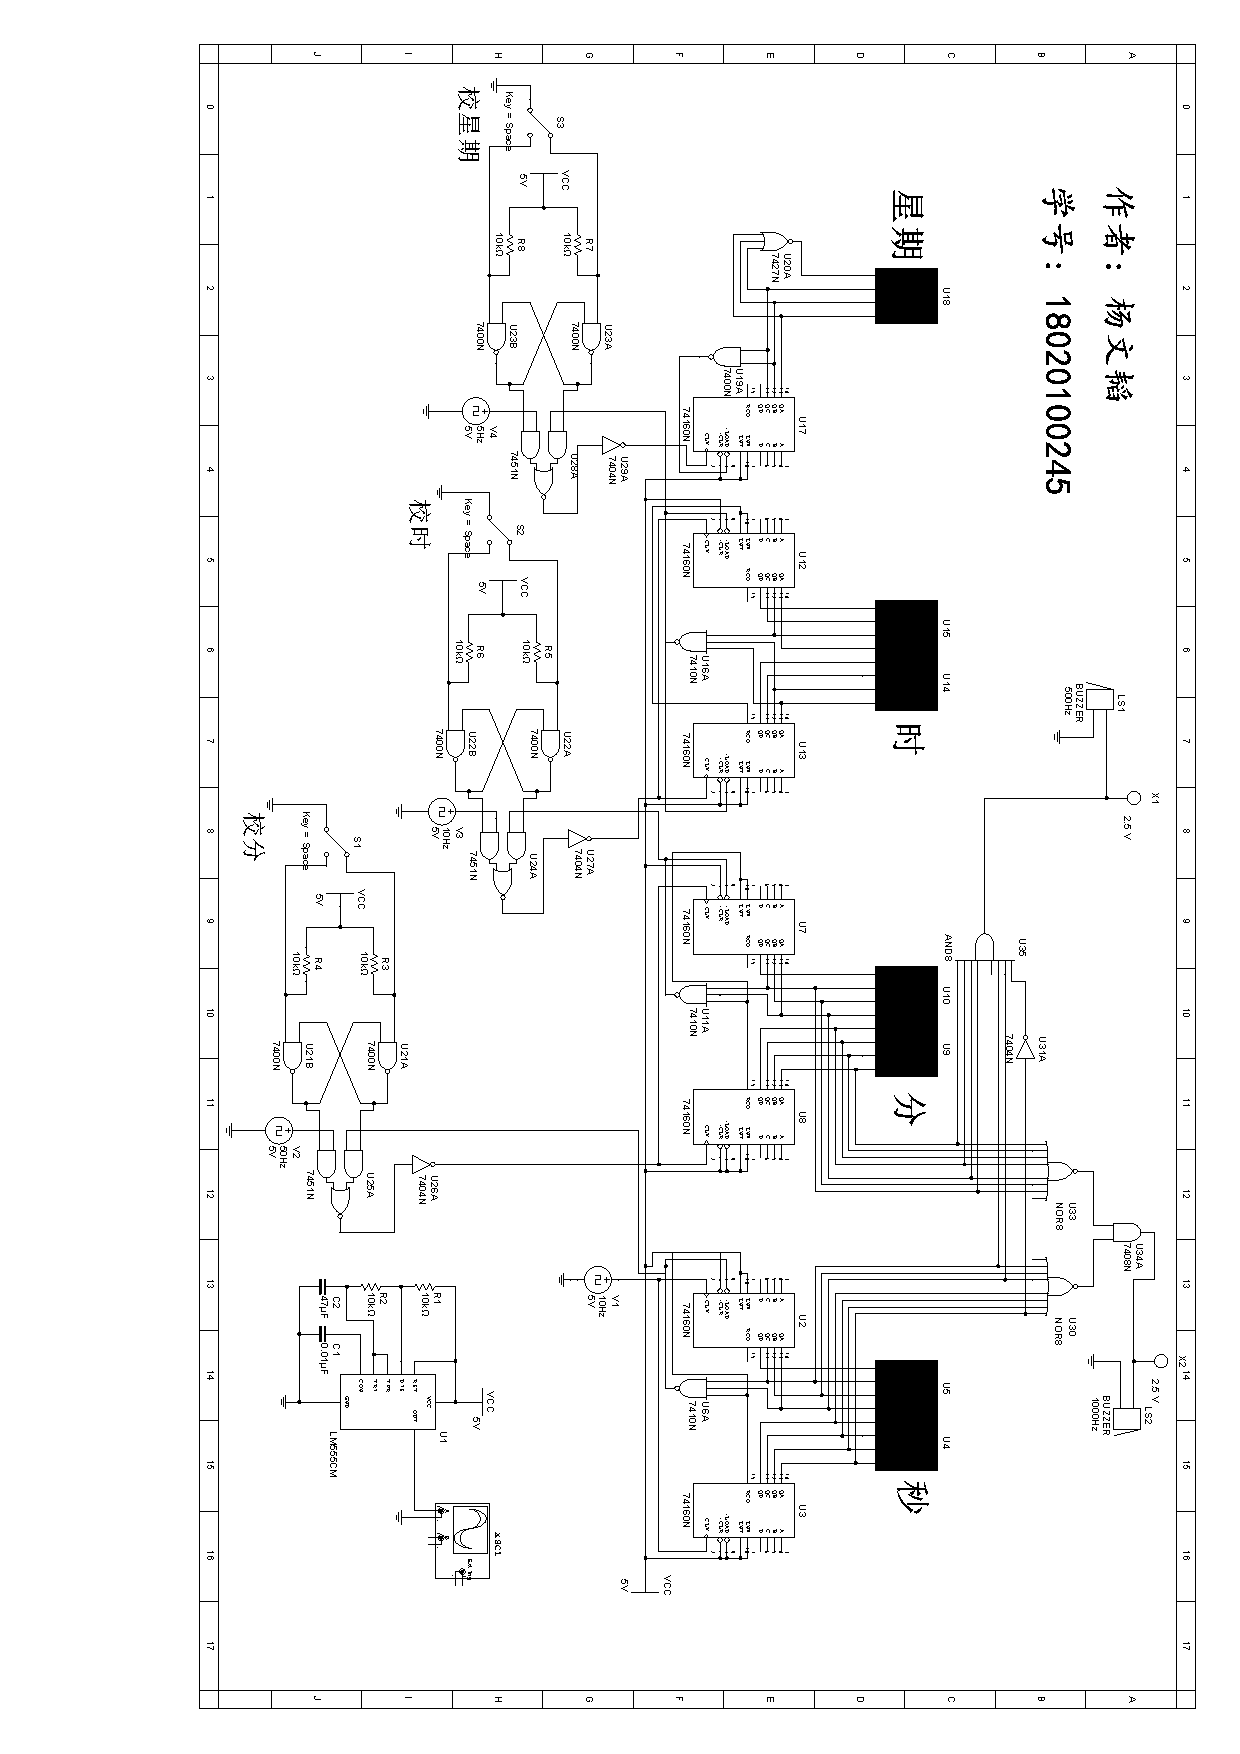
\includegraphics[width=10.5cm]{figure/DigitalClock}
	\caption{仿真电路图}\label{fig:DigitalClock}
\end{figure}
	
\end{document}
%%%%%%%%%% 结束 %%%%%%%%%%